\chapter{Raw and XML digital signature and encryption}
On the previous chapter we have seen digital documents, which biggest
security part is the signature. For that, PDFs are using the PKCS\#7 
standard, and XMLs are using the XML-DSig standard. In this chapter we 
will see how these standards work.
\section{PKCS\#7 and CMS}
PKCS\#7 is the original standard from RSA, since RSA was the owner of
the RSA algorithm, they wanted also to define standards about the
usage of the algorithm, and they had a series of standards named PKCS.

PKCS\#7 was a standard for secure enveloping (secure is a generic
term, it means authentication, integrity, confidentiality and so on),
at some point in v1.5, the work was shared with IETF and later RSA
stopped the development of PKCS\#7 and the rest was developed directly
by IETF which renamed it in CMS (Cryptographic Message Syntax).

\begin{boxH}
  CMS is a \textbf{secure envelop} that allows data authentication,
  integrity and, optionally, privacy, with symmetric or asymmetric
  algorithms, depending on the kind of application.
\end{boxH}

It also supports multiple signatures (hierarchical or parallel) on the
same object, and it can include the certificates (and can include also
revocation info) to verify the signature to be a self contained
object, where the signature envelops the data and the certificate 
needed to verify the signature.

PKCS\#7 and CMS are raw format, in the sense that they consider
generic data that are just binary blob/stream (sequence of bit), and
this sequence of bits is encapsulated in a secure container. It is
very important because it is the only standard that permits to sign
and encrypt any kind of data, and it is a recursive format, which is
important because there is not one format which is providing signature
and encryption, but it is possible to achieve that by making first
encryption, then that object becomes a generic data which is inserted
in another container which is providing the signature.

PKCS\#7 and CMS are defined using ASN.1 (Abstract Syntax Notation 1)
with different encoding rules (Basic Encoding Rule, BER, for most of
the standard and the Distinguished Encoding Rule, DER, only for the
signed attributes and authenticated attributes).

Initially, it was defined by RSA and then it evolved over the time:
\begin{itemize}
  \item RFC-2630 (Jun ‘99): fully compatible PKCS\#7 1.5 but with
    key-agreement (DH algorithm) and pre- shared keys
  \item RFC-3369 (Aug ‘02): adds password-based keys and an extension
    schema for generic key management and it splits the document into
    two RFCs (one for the basic structure of secure envelop and the
    other for the algorithms, so that they can evolve independently
    for the secure container)
  \item RFC-3852 (Jul ‘04): it is just a generalization, an extension
    that supports generic certificates (not very frequent to use
    something different from X.509 is used)
  \item RFC-5652 (Sep ‘09): clarifications about multiple signatures
\end{itemize}

\subsection{Algorithms for CMS}
The allowed algorithms are documented in RFC-3370:
\begin{itemize}
  \item Digest MD5, SHA-1: quite old
  \item Signature RSA, DSA (insecure without elliptic curve)
  \item Key management:
    \begin{itemize}
      \item DH for key agreement
      \item RSA for transport
      \item For symmetric wrapping 3DES and RC2
      \item Derivation PBKDF2
    \end{itemize}
  \item For encryption: 3DES-CBC, RC2-CBC
  \item For MAC: HMAC-SHA1
\end{itemize}
These algorithms were very basic and quite old, but with new RFCs the
situation improved:
\begin{itemize}
  \item For encryption: CAST-128, IDEA, AES, Camellia, SEED
  \item For digital signature RSASSA-PSS, so a better schema is used
    (more resistant to attacks)
  \item For encryption and digest: GOST (the one used in Russia)
  \item AES-CCM and AES-GCM for authenticated encryption (be aware: it
    does not provide nonrepudiation since it is not digital signature)
  \item Boneh-Franklin and Boneh-Boyen for Identity-Based Encryption,
    it is a new kind of encryption in which the key is based on the
    identity of the actors (e.g., IP address)
  \item ECC and SHA-2 family is supported
  \item RSA-KEM and RSAES-OAEP for key transport
\end{itemize}

\subsection{CMS structure}
The CMS structure is shown in figure \ref{fig:cms structure}, and
basically one CMS component, the \textbf{contentInfo}, which contains
inside the contentType and the content itself.

This allows for encapsulation, because the content can be another CMS 
object(contentInfo) allowing for a recursive structure. 

\begin{figure}[H]
  \centering
  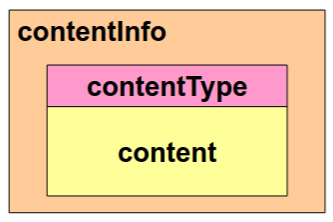
\includegraphics[width=0.4\textwidth]{img/cms structure.png}
  \caption{CMS structure}
  \label{fig:cms structure}
\end{figure}

\subsection{CMS content type}

There are different contentType available:

\begin{itemize}
  \item \textbf{data}: A generic sequence of bytes, serving as the
    base content.
  \item \textbf{signedData}: The data accompanied by one or more
    digital signatures (1..N), allowing parallel signing. In this
    case, all the signatures are computed over the same data,
    without any particular order.
  \item \textbf{envelopedData}: The data encrypted using a symmetric
    algorithm, with the symmetric key encrypted for the intended
    recipient(s). This means that the symmetric key is present in
    the data, but only the intended recipient(s) can decrypt it,
    because it is encrypted with their public key.
  \item \textbf{authenticatedData}: The data, a Message
    Authentication Code (MAC), and an encrypted key for
    recipient(s). Same drill as with envelopedData, the key is
    present and encrypted with the public key of the intended 
    recipient(s).
  \item \textbf{digestedData}: The data along with its cryptographic
    digest for integrity verification.
  \item \textbf{encryptedData}: The data encrypted using a symmetric
    algorithm, providing confidentiality.
\end{itemize}

\subsection{CMS signed data}
It is used to implement digital signature, so the content type is
signedData, while the actual content has:
\begin{itemize}
  \item \textbf{version}: the version of the object, not the version
    of the CMS standard.
  \item \textbf{digestAlgorithms}: this is a list: since the signed data
    can be signed by different people, they may be using different
    algorithms to sign the data. The algorithms must be listed before
    the signature to make them known to the verifier before the data is
    actually read. This allows to compute the digest in parallel while 
    the data is being read.
  \item \textbf{encapContentInfo}: the informations about the content
    that is being encapsulated.

  \item \textbf{certificates}: this is optional, these are all the certificates
    of the signers, and typically all the certificate chain for each
    signer.
  \item \textbf{crls}: this is optional, it is used to verify that
    each certificate was valid at the moment of the signature. 
  \item \textbf{signerInfo}: a block for each signer and each block is
    composed by a version number, the distinguish name of the issuer
    of the certificate (so the CA) + the Serial Number of the
    certificate related to this specific signature (because a generic
    signer could have more than one certificate), finally you have the
    digest encrypted with the private key corresponding with this
    public key.
\end{itemize}

\begin{figure}[H]
  \centering
  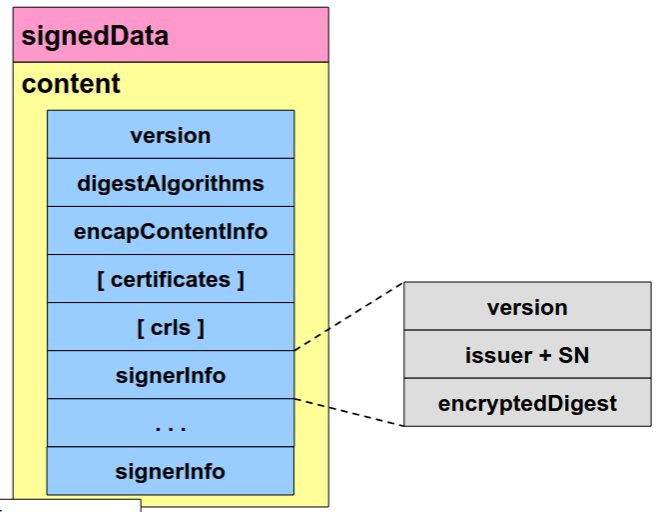
\includegraphics[width=0.4\textwidth]{img/cms signed data.png}
  \caption{CMS signed data}
\end{figure}

\subsection{CMS enveloped data}
The enveloped data, on the contrary, provides encryption.
\begin{itemize}
  \item \textbf{version}: to know which kind of object we are
    considering.
  \item \textbf{encryptedContentInfo}: which is a block composed of a
    contentType (contains the type of content you will find after the
    decryption), the description of the algorithm used for the
    encryption, and finally the encrypted content. Notice that only
    one algorithms can be specified, meaning that one can sign with
    different algorithms but can encrypt with only one.
  \item \textbf{recipientInfo}: this is the list of possible
    recipients (or people that are authorized to perform the
    decryption), because for each possible recipient there is one
    block that contains the version, the issuer + the serial number of
    the certificate (as in the previous case), the encryption
    algorithm used to encrypt the symmetric key (e.g. RSA), and
    finally the encrypted key.
\end{itemize}

\begin{figure}[H]
  \centering
  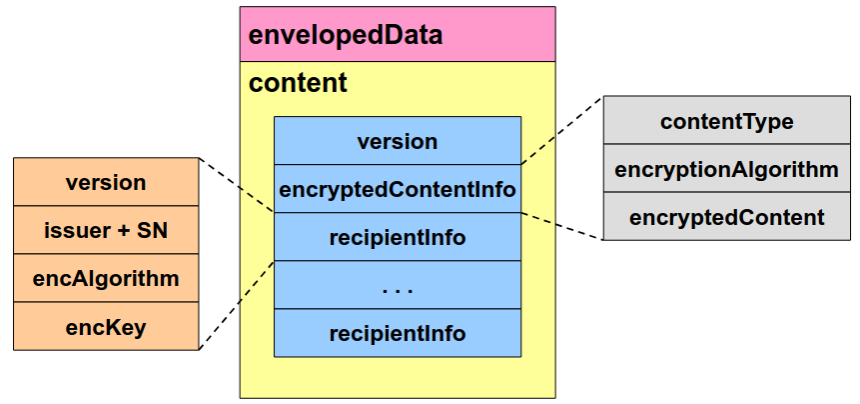
\includegraphics[width=0.5\textwidth]{img/cms enveloped data.png}
  \caption{CMS enveloped data}
\end{figure}

\section{XML digital signature}

XML signature is important because there are several practical systems
that make use of XML to represent generic data.

XML signature is a standard promoted not by IETF but the W3C with the
cooperation by IETF but since most of the XML standardization is done
in W3C they were the initiator. Even if the standard is named XML
signature note that it covers not only digital signature but also a
MAC. One standard here covers both things. With respect to the signed
data, it provides authentication, integrity, and non-repudiation
(optional, only if the signature is performed with asymmetric crypto
and associated to an X.509 certificate).

Another desirable feature that the XML signature provides is the 
independence from the transport layer or any storage technique.

\subsection{XML Signature – Standard}

\textbf{1st Edition (Recommendation):}
\begin{itemize}
  \item Initial version:
    \url{www.w3.org/TR/2002/REC-xmldsig-core-20020212/}
  \item RFC-3275 specifies its use.
  \item Latest version of v1 available at:
    \url{http://www.w3.org/TR/xmldsig-core/} (currently v1.1, dated
    11-Apr-2013).
\end{itemize}

\textbf{2nd Edition:}
\begin{itemize}
  \item Available at: \url{https://www.w3.org/TR/xmldsig-core2/}.
  \item Latest version published on 23-Jul-2015.
\end{itemize}

\subsection{XML Digital Signature – Namespace}
To identify the elements that are present in the standard, there is
the need of specific identifiers. In XML terminology it is
namespace. Specific identifiers are can be found at
\url{http://www.w3.org/2000/09/xmldsig#}. 
An example of the namespace is shown in figure \ref{fig:xml
signature namespace}. It is named \texttt{dsig}, which is providing
entries to the defined url.

It is common, sing XML is very verbose, to define an abbreviation,
by using the ENTITY command. It means that after that is possible to
use the abbreviation with the \texttt{\&} in the front, so that is
not necessary to repeat that long string.


\begin{figure}[H]
  \centering
  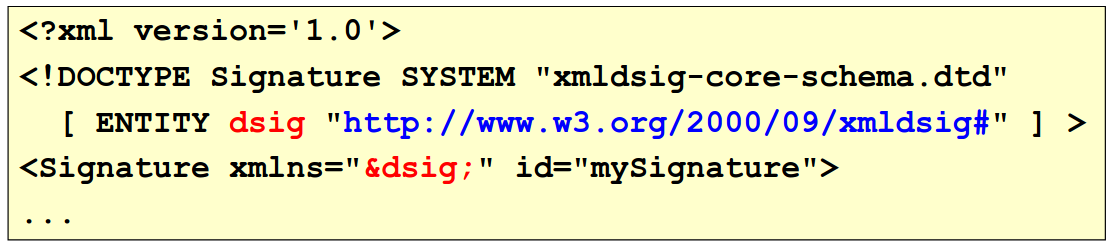
\includegraphics[width=0.5\textwidth]{img/xmldsig namespace.png}
  \caption{XML Signature Namespace}
  \label{fig:xml signature namespace}
\end{figure}

\subsection{General Characteristics of XMLdsig}

The XML Signature framework offers versatile signing capabilities for
XML and non-XML objects.

The signed object may be:
\begin{itemize}
  \item Internal (contained within the signature) or external
    (only referenced via a URI).
  \item XML (native object) or non-XML (encapsulated object with an
    XML signature).
\end{itemize}

It supports different signature levels for the same content, with
flexible semantics:
The main difference with reference to a CMS signature is the
flexibility of the semantics, in fact the XML signature can be:
\begin{itemize}
  \item Signed.
  \item Co-signed.
  \item Witnessed.
  \item Notarized.
\end{itemize}

However, XMLdsig does not address key creation or certification,
focusing solely on signing and integrity verification.

\subsection{Signature types}
The different formas have been already briefly discussed in section 
\ref{sec:formats of signed documents}, and are basically the same in
XML. With an enveloping signature, the XML object in stored inside a
XML signature object, while with an enveloped signature the XML object 
reserve some space to store the signature. A detached signature in XML
is basically and URI which points to the signature.
\begin{figure}[H]
  \centering
  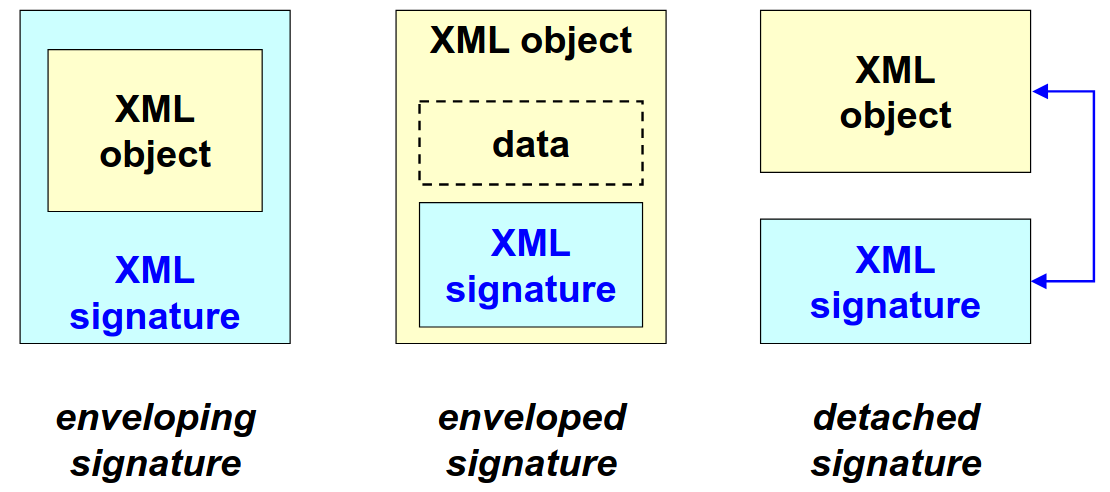
\includegraphics[width=0.4\textwidth]{img/xml signature types.png}
  \caption{XML Signature Types}
\end{figure}

\subsection{Canonicalization}
When dealing with XML, there's a problem that have to be dealt with: 
there are many equivalent forms for the same data. Take a look at this
example:
\begin{listing}[H]
  \centering
  \begin{minted}{xml}
 <person id="12345" name="Antonio"/>
 <person name="Antonio" id="12345"/>
 <person name="Antonio" id="12345"></person>
  \end{minted}
  \caption{Equivalent XML}
\end{listing}
All the three forms are equivalent, but if you compute the hash of
each of them, you will get different results, due to the different 
format. Another example could be empty spaces, which are not relevant 
for the XML parser, but they are relevant for the hash computation,
and so on.

In those case logical equivalence should be the same as actual one in
terms of signature.

\subsubsection{Canonicalization algorithms}

Canonicalization algorithms are used to transform the XML document in 
a canonical form, so that the signature is always the same, no matter 
the format of the XML document.  This is done by creating a physical 
representation of the XML document, by representing the XPath node set 
as an octet sequence.

The algorithms changed over the time, the default being canonical XML
1.0 which follows that specification, eventually with comments (if
comments are appropriate or not inside the XML document) but the
preferred version is the most recent one called canonical XML 1.1:
the comments should be deleted when computing the signature or should
be included in the computation of the signature? There are two
different canonicalization ways according to the fact that comments
are included or not.

\subsubsection{Canonicalization process}
The canonicalization process is specified at
\url{http://www.w3.org/TR/xml-c14n.html} and is as follows:
\begin{enumerate}
  \item encode the document in UTF-8
  \item normalize line breaks to \#xA(10), before parsing, after all some
    use line feed, some use carriage return, some use both
  \item normalize attribute values, as if by a validating processor,
    for example remove the leading zeroes in the numbers
  \item replace character and parsed entity references(replace
    references with the actual content)
  \item replace CDATA sections with their character content
  \item remove XML declaration and DTD
  \item convert empty elements to start-end tag pairs
  \item normalize whitespace outside of the document element and
    within start and end tags
  \item retain all whitespace in character content (but characters
    removed during line feed normalization), meaning that spaces in
    strings are retained
  \item set attribute value delimiters to quotation marks(single
    quotes became double quotes)
  \item replace special characters in attribute values and character
    content by character references
  \item remove superfluous namespace declarations from each element
  \item add default attributes to each element
  \item impose lexicographic order on the namespace declarations and
    attributes of each element
\end{enumerate}

\subsection{Structure of XML signature}
The general structure of an XML signature is shown in figure 
\ref{fig:xml signature structure}, and as you can see can have an
optional identifier. Keep in mind that SignatureValue is computed over
the SignedInfo.

\begin{figure}[H]
  \centering
  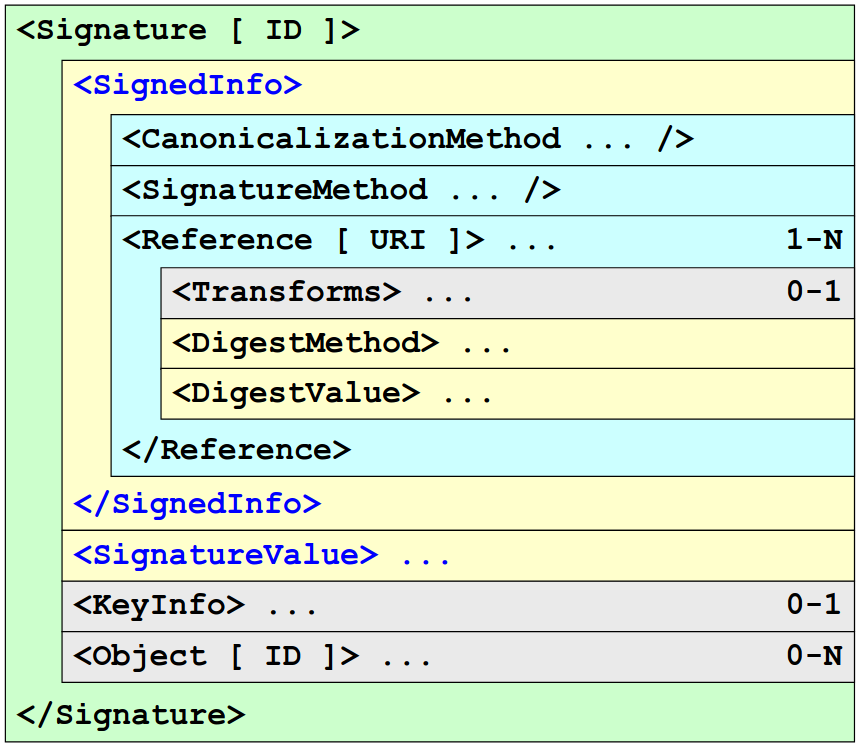
\includegraphics[width=0.5\textwidth]{img/xml signature structure.png}
  \caption{XML Signature Structure}
  \label{fig:xml signature structure}
\end{figure}

\subsubsection{SignedInfo}

The \texttt{SignedInfo} element is a crucial component of an XML
signature and always appears as the first element. Its main components
include:

\begin{itemize}
  \item \textbf{CanonicalizationMethod:} A data normalization
    technique applied before generating the signature.
  \item \textbf{SignatureMethod:} Specifies the algorithm used for
    signature generation, such as RSA+SHA1.
  \item \textbf{Reference [URI]:} A pointer to the actual data that
    has been signed. The 1:N cardinality means that one can have
    just one signature for n objects or n references when you want
    to sign a group of documents.
    \begin{itemize}
      \item \textbf{Transforms (optional):} Data transformations
        applied before signing, such as selecting elements via
        XPath.
      \item \textbf{DigestMethod:} The hash algorithm employed,
        e.g., SHA1.
      \item \textbf{DigestValue:} The computed hash value of the
        referenced data.
    \end{itemize}
\end{itemize}

\subsubsection{Reference URI}

The \texttt{Reference URI} is a pointer to an element that has been
signed. Its usage depends on the context and signature type:

\begin{itemize}
  \item \textbf{Omission:} The \texttt{URI} may be omitted for at
    most one \texttt{Reference} or \texttt{Manifest} component if
    the signed element is unambiguously determined by the context
    (e.g., an application-level message signature).
  \item \textbf{Null URI (URI=""):} Used to generate an enveloped
    signature.
  \item \textbf{Self URI (URI="\#id"):} Used to generate an
    enveloping signature.
  \item \textbf{External URI (e.g., URI="http://..."):} Used to
    generate a detached signature.
    \begin{itemize}
      \item When an external URI is specified, follow any redirects
        (status 3xx) until reaching the body of a positive response
        (status 200).
    \end{itemize}
\end{itemize}

\subsubsection{Reference Type}

A reference can point to various element types, each serving a
specific purpose:

\begin{itemize}
  \item \textbf{Object:} Refers to a generic object.
  \item \textbf{SignatureProperty:} Points to a signature attribute,
    such as date and time or the HSM identifier. The type is
    specified as \texttt{Type="\&dsig;SignatureProperties"}.
  \item \textbf{Manifest:} Represents a set of references, useful
    for grouping related elements. The type is specified as
    \texttt{Type="\&dsig;Manifest"}.
\end{itemize}

\subsubsection{Manifest}
It is a list of references external to SignedInfo but pointed to by
the same. Basically the manifest is somewhere in the XML tree and is
pointed to by the SignedInfo, as you can also see from figure 
\ref{fig:xml manifest}.

There is a conceptual difference to understand why there is a manifest
rather than having the pointer to the object directly inside
signedInfo.
Each reference in SignedInfo is subject to the validation procedure;
it means that if anyone is invalid (e.g., inaccessible URI, wrong
DigestValue) then the whole signature is invalid. If the object is put
inside SignedInfo and validation fails, the whole signature must be
rejected. On the other hand, any reference in the manifest is not
individually validated since the procedure considers only the Manifest
as a whole. This means that it is possible to check that the signature
is the correct digest of the manifest but not where the manifest is
pointing because the manifest is here, it is signed but then the
manifest is pointing, for example, to three external documents,
beacuse it out of scope checking the integrity of the linked
documents, as it's the application's responsibility to do so.

It is possible to notice that in the SignedInfo there is a reference
to a URI which is towards an object, and the type is “signature of a
manifest”. Then, at some point there is an object which has the same
identifier (\textbf{myManifest}) as the reference, saying “this is the
thing that was signed”, and inside the manifest there are several
references. So the digestValue in the Reference is the digest of the
list contained in the manifest. So, we are only checking that the SHA1
is correct, but then each of these references contains a method and a
value. So, if you want you can verify also if those objects have
changed or not. But this is not what is done by XML signature.

This approach provides flexibility but also introduces risks. If you
rely on XML signatures without careful implementation, you might
assume that having a digital signature guarantees protection. However,
if your implementation references objects indirectly through a
manifest instead of directly, someone could potentially alter values
within the references without detection. The automatic XML signature
process only verifies that the SHA1 hash in the \texttt{DigestValue} field
matches the overall manifest. It does not follow the links to validate
individual elements. 


\begin{figure}[H]
  \centering
  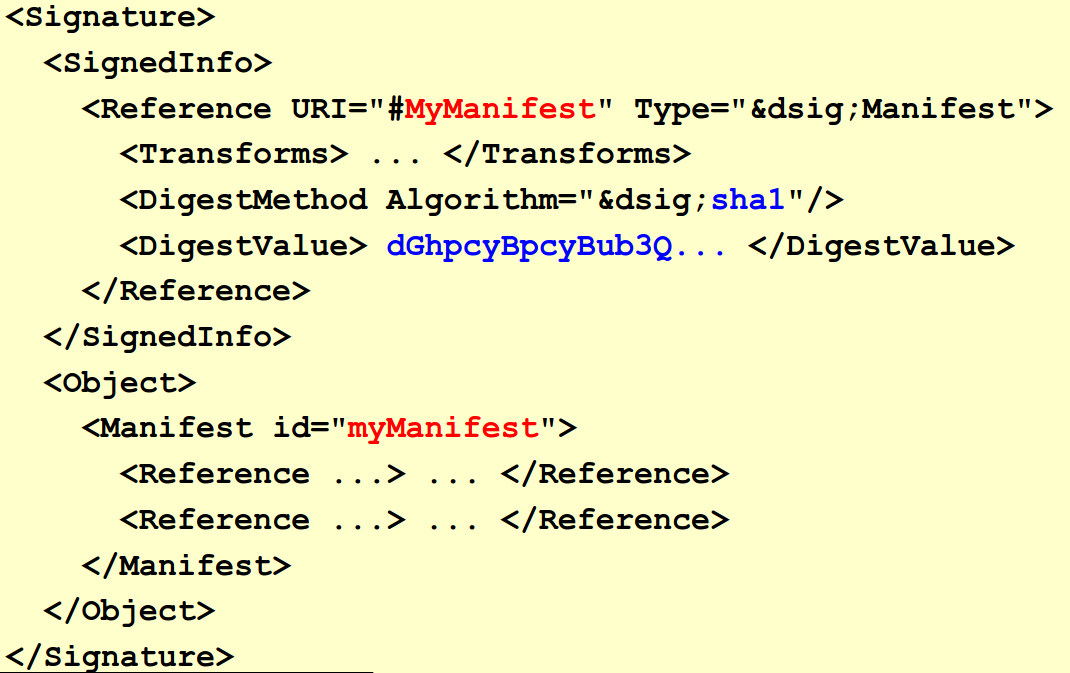
\includegraphics[width=0.5\textwidth]{img/xml manifest.png}
  \caption{XML Signature Manifest}
  \label{fig:xml manifest}
\end{figure}


\subsubsection{Transforms}
The transforms may contain one or more \mintinline{xml}{<Transform>}
tags to be applied sequentially before computing the digest. That’s
important otherwise you risk computing the wrong digest. Possible
transformations are:
\begin{itemize}
  \item EnvelopedSignature: the one which is compulsory and may be
    implemented via Xpath
  \item XPath transform: compulsory
  \item XSTL (X Stylesheet) transform optional
  \item Other transformations may be used but they are quite
    deprecated because they are not native in XML
\end{itemize}

XPath plays a crucial role by allowing you to specify which parts of
an XML object should be included in the signature. This flexibility is
important depending on what you are signing—whether every part is
relevant or if certain elements are variable and not meaningful. 

For example, imagine signing a file that includes an access control
section recording when the file was last accessed. This timestamp is
likely to change over time and isn’t relevant to verifying the file’s
integrity. What matters is ensuring that the file’s content remains
unchanged. Including such auxiliary information in the signature
computation would require re-signing the file every time it’s
accessed. 

Using XPath, you can define precisely which parts of the object should
be included in the digest computation, enabling efficient and
meaningful signatures.

\subsubsection{DigestMethod and DigestValue}

The \texttt{DigestMethod} specifies the cryptographic hash algorithm
used to generate the input for the signature process. One compulsory
algorithm is \texttt{SHA1}, which is identified by the URI
\texttt{http://www.w3.org/2000/09/xmldsig\#sha1}. This algorithm
operates on a byte stream as input.

The handling of input depends on the output of the URI dereference and
any \texttt{Transforms} applied:
\begin{itemize}
  \item If the result is a set of XPath nodes, the byte stream is
    generated using Canonical XML (\texttt{XML-C14N}).
  \item If the result is already a byte stream, the digest is
    computed directly.
\end{itemize}

The \texttt{DigestValue} represents the value obtained after applying
the \texttt{DigestMethod}. This value is encoded using Base64 for
inclusion in the XML signature structure.

\subsubsection{SignatureMethod}

The \texttt{SignatureMethod} specifies the algorithm used to generate
the digital signature. A complete list of supported algorithms is
available at
\url{https://www.w3.org/TR/xmldsig-core2/\#sec-SignatureMethod}.

Mandatory algorithms include:
\begin{itemize}
  \item For digest operations: \texttt{SHA-256} (recommended) and
    \texttt{SHA1} (discouraged).
  \item For MAC operations: \texttt{HMAC-SHA-256} (recommended) and
    \texttt{HMAC-SHA1} (discouraged), with an optional parameter to
    specify the truncation length.
  \item For digital signatures: \texttt{RSAwithSHA256},
    \texttt{ECDSAwithSHA256}, and \texttt{DSAwithSHA1} (supported
    for verification only).
\end{itemize}

The signature value is the value base64 encoded. This is not computed
directly over the referenced data, but on their digest (because we
compute the signature of SignedInfo).

\begin{figure}[H]
  \centering
  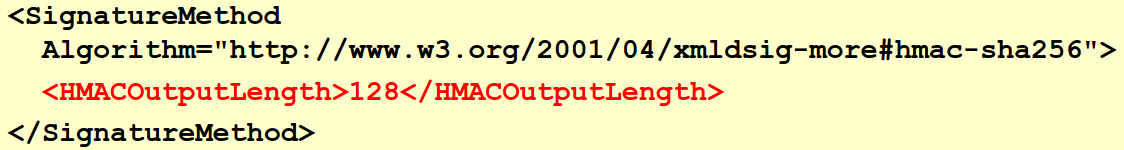
\includegraphics[width=0.6\textwidth]{img/xml signature value.png}
  \caption{XML Signature Method}
\end{figure}

\subsection{Security requirements}
XML security mechanisms address several key requirements:

\textbf{Confidentiality} is provided by TLS and XML Encryption but not
directly by XML Signature.

\textbf{Message Authentication} ensures message integrity and verifies
the creator using MAC or digital signatures. However, it does not
confirm the sender's identity.

\textbf{Sender/Receiver Authentication} verifies the identities of
both parties, achieved through TLS client authentication. This does
not ensure the authenticity of the message creator.

To guarantee that the signer is also the sender, we may use
the same X.509 certificate as in SOAP-DSIG or SOAP-TLS
( in this case, the \mintinline{xml}{<ds:KeyInfo>} element may be
omitted)

\subsection{Weaknesses}

XML Signature implementations have some potential vulnerabilities:

A \textbf{malicious receiver} could falsely claim to have received a
message multiple times, even if it was sent only once. To counter
this, a nonce, such as a timestamp, should be added to the message.

A \textbf{malicious receiver} might forward the signed message to a
third party, who could then falsely claim to have received it directly
from the sender. Including the intended receiver's identity within the
signed message can mitigate this risk.

Possible countermeasures involve adding both a timestamp and receiver
identity to the signed body of the message.

\subsection{Example of a (detached) XML signature}

An example of a detached XML signature is shown in listing
\ref{lst:xml signature example}. The signature algorithm is DSA with 
SHA-1, and the canonicalization algorithm is XML-C14N, as specified by
the transform algorithm. The signature is deatached because the URI 
points to an external document.

\begin{listing}[H]
  \centering
  \begin{minted}{xml}
  <Signature Id=“Lioy_dsig_081026173907” xmlns=“http://www.w3.org/2000/09/xmldsig#”>
    <SignedInfo>
      <CanonicalizationMethod Algorithm= "http://www.w3.org/TR/2001/REC-xml-c14n-20010315"/>
      <SignatureMethod Algorithm= "http://www.w3.org/2000/09/xmldsig#dsa-sha1"/>
      <Reference URI="http://www.sito.it/doc.xml"/>
        <Transforms>
          <Transform Algorithm= "http://www.w3.org/TR/2001/REC-xml-c14n-20010315"/>
        </Transforms>
        <DigestMethod Algorithm= "http://www.w3.org/2000/09/xmldsig#sha1"/>
        <DigestValue>j61wx3rvEPO...</DigestValue>
      </Reference>
    </SignedInfo>
    <SignatureValue>JK34s...</SignatureValue>
    <KeyInfo>
      <X509Data>
        <X509Certificate>
          MII...AABvi
        </X509Certificate>
      </X509Data>
    </KeyInfo>
  </Signature>
  \end{minted}
  \caption{XML Signature Example}
  \label{lst:xml signature example}
\end{listing}

\section{XML Encryption}
XML encryption is a standard to represent encrypted data while also
specifying the encryption and decryption process. It is a W3C 
standard with different versions, the first one being the 1.0, and the 
latest, and recommended, one being the 1.1.

There are 4 different possible encryption scopes:
\begin{itemize}
  \item a XML element
  \item the content of an XML element
  \item a whole XML document
  \item just a portion: an EncryptedData or EncryptedKey element (this
    is named super-encryption)
\end{itemize}
The result of any of these operations is always an XML encryption
element, which may contain the encrypted data. So, in this case, there
is a detached encryption. It means that the encrypted content is in
some place, and in XML encryption there is everything needed to
decrypt that content.
\subsection{Syntax}

The syntax of XML Encryption (\texttt{XMLenc}) includes the following
components:

\begin{itemize}
    \item \textbf{EncryptedType}: This is the abstract type used for
      both \texttt{EncryptedData} and \texttt{EncryptedKey}.
    
    \item \textbf{EncryptionMethod}: Specifies the algorithm employed
      for encryption.
    
    \item \texttt{ds:KeyInfo}: Contains details about the key used in
      the encryption process.
    
    \item \textbf{CipherData}: This includes either:
    \begin{itemize}
        \item \texttt{CipherValue}: Base64-encoded encrypted data.
        \item \texttt{CipherReference}: A pointer to the encrypted data.
    \end{itemize}
    
    \item \textbf{EncryptionProperties}: Provides supplementary
      information about the generation of the encrypted data.
    
    \item \texttt{Id} (optional): A unique document identifier.
    
    \item \texttt{Type} (optional): Specifies the type of document,
      such as an element or content.
    
    \item \texttt{MimeType} (optional): Indicates the MIME type of the
      encrypted data.
\end{itemize}

\subsection{XML Encryption: Required Algorithms}

In version 1.0 of XML Encryption, the following algorithms were used:

\begin{itemize}
    \item \textbf{Encryption}: 3DES-CBC (for backward compatibility), but also AES-128/256-CBC.
    \item \textbf{Key Transport}: RSA-v1.5, RSA-OAEP (RSA Optimal Encapsulation, preferred). Used to give the encrypted content to the recipient.
    \item \textbf{Symmetric Key Wrap}: 3DES (for backward compatibility, should never be used), AES-128, or AES-256 KeyWrap.
    \item \textbf{Digest}: SHA1, SHA256 (recommended). The digest is not a signature but is useful.
    \item \textbf{Authentication}: XMLdsig.
\end{itemize}

In version 1.1, additional algorithms were introduced, including support for authenticated encryption:

\begin{itemize}
    \item \textbf{Encryption}: 3DES-CBC, AES-128/256-CBC, AES128-GCM.
    \item \textbf{Key Derivation}: ConcatKDF. In the previous versions, PKDF2 or HKDF were used, but XMLenc uses ConcatKDF.
    \item \textbf{Key Transport/Key Agreement}: RSA-OAEP, ECDH.
    \item \textbf{Symmetric Key Wrap}: 3DES, AES-128, or AES-256 KeyWrap.
    \item \textbf{Digest}: SHA1 (discouraged), SHA256.
\end{itemize}

\subsection{Examples of XML Encryption}
Let's now look at some examples of XML encryption. We will take as
reference listing \ref{lst:xml payment info}, which is an XML document 
containing payment information of a user.

\begin{listing}[H]
  \centering
  \begin{minted}{xml}
  <?xml version='1.0'?>
  <PaymentInfo xmlns='http://cards.org/payment'>
    <Name>Gianni Pautasso</Name>
    <CreditCard Limit='1,500' Currency='EUR'>
      <Number>4091 2450 0288 5657</Number>
      <Issuer>MyBank/Issuer>
      <Expiration>06/10</Expiration>
    </CreditCard>
  </PaymentInfo>
  \end{minted}
  \caption{XML Payment Info}
  \label{lst:xml payment info}
\end{listing}

One possibility, if we want to protect sensitive data, is to encrypt
the whole \texttt{CreditCard} XML tag, as well as its content, as
shown in figure \ref{fig:xml enc ex 1}. In this case, the encryption
algorithm is not specified, its not compulsory after all, which means
that the knowledge of which algorithm to use is delegated to the 
application that will decrypt the data, as well as the key agreement.

Another possibility is to leave most of the \texttt{CreditCard} data
in clear, and encrypt only the credit card number, as shown in figure
\ref{fig:xml enc ex 2}. 

A third possibility is to encrypt the whole XML document, as shown in 
figure \ref{fig:xml enc ex 3}. In this case, it is necessary to
specify the MIME type of the encrypted data explicitly, unlike the
previous example where the encrypted part was basically just data. 

Until now, the encryption algorithms were not specified, but it is 
possible to do so, as shown in figure \ref{fig:xml enc ex 4}, which is
basically the previous example with the addition of the encryption 
algorithm. A key must also be specified. In this case, the standard
from XMLdsig is used to give a name to this key, "Alice-Bob" in this
case, which is just something meaningful to the two parties involved.

\begin{figure}[H]
  \centering
  \subfloat[XML Encryption Example 1]{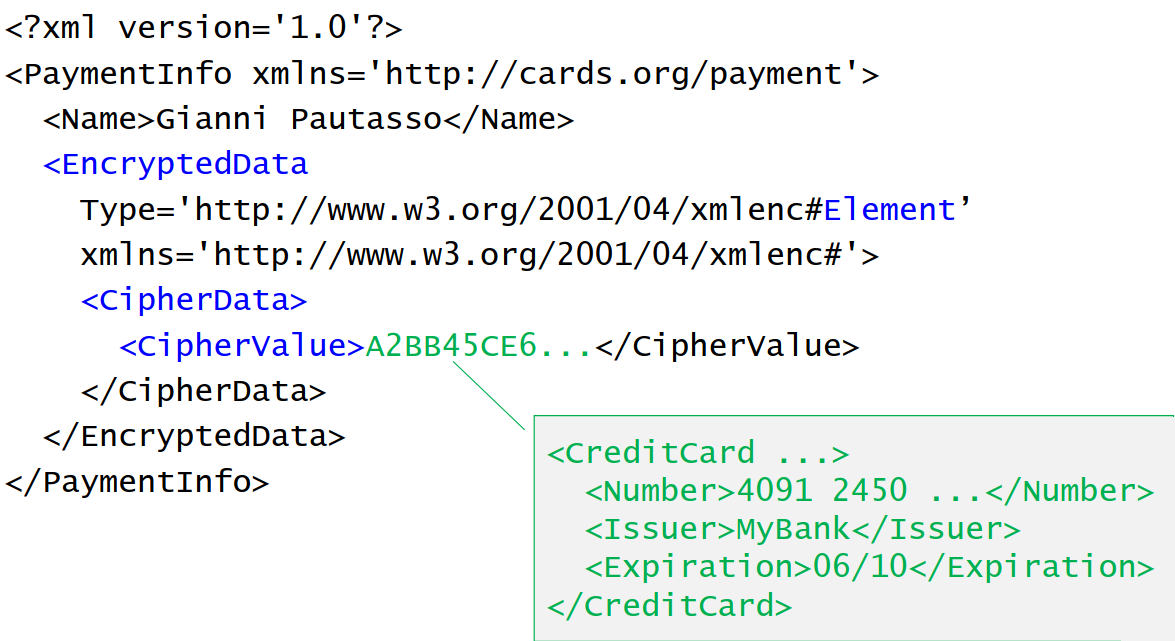
\includegraphics[width=0.48\textwidth]{img/xml encryption ex 1.png}\label{fig:xml enc ex 1}}
  \hfill
  \subfloat[XML Encryption Example 2]{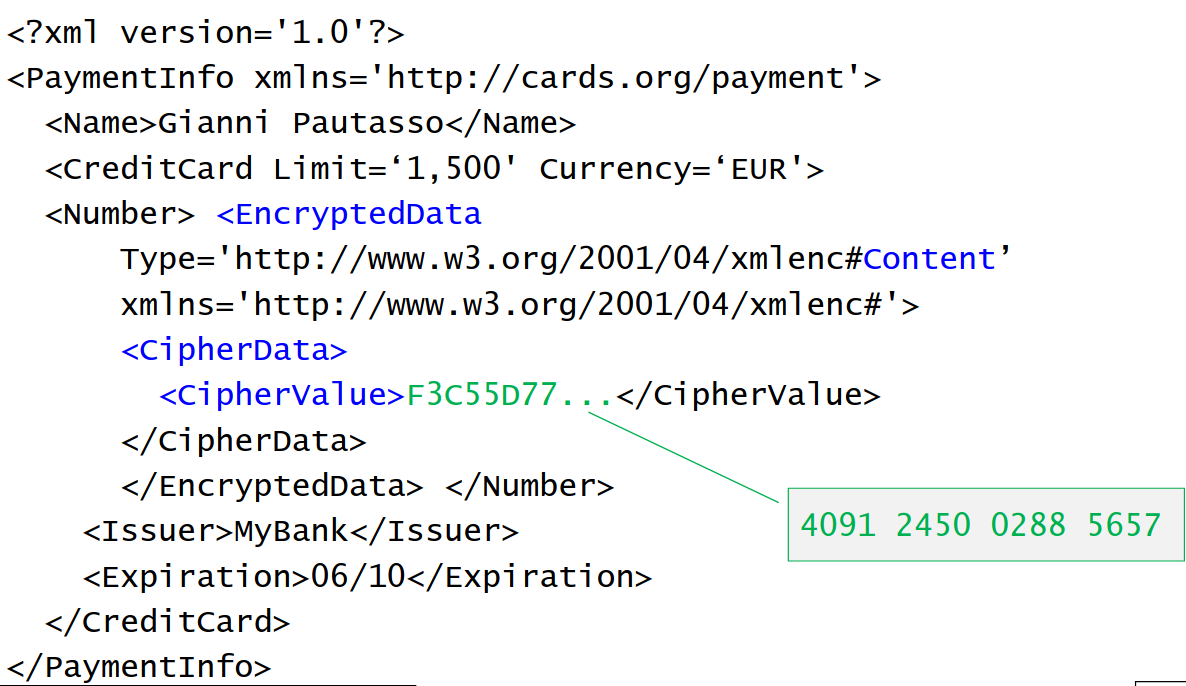
\includegraphics[width=0.48\textwidth]{img/xml encryption ex 2.png}\label{fig:xml enc ex 2}}
  \hfill
  \subfloat[XML Encryption Example 3]{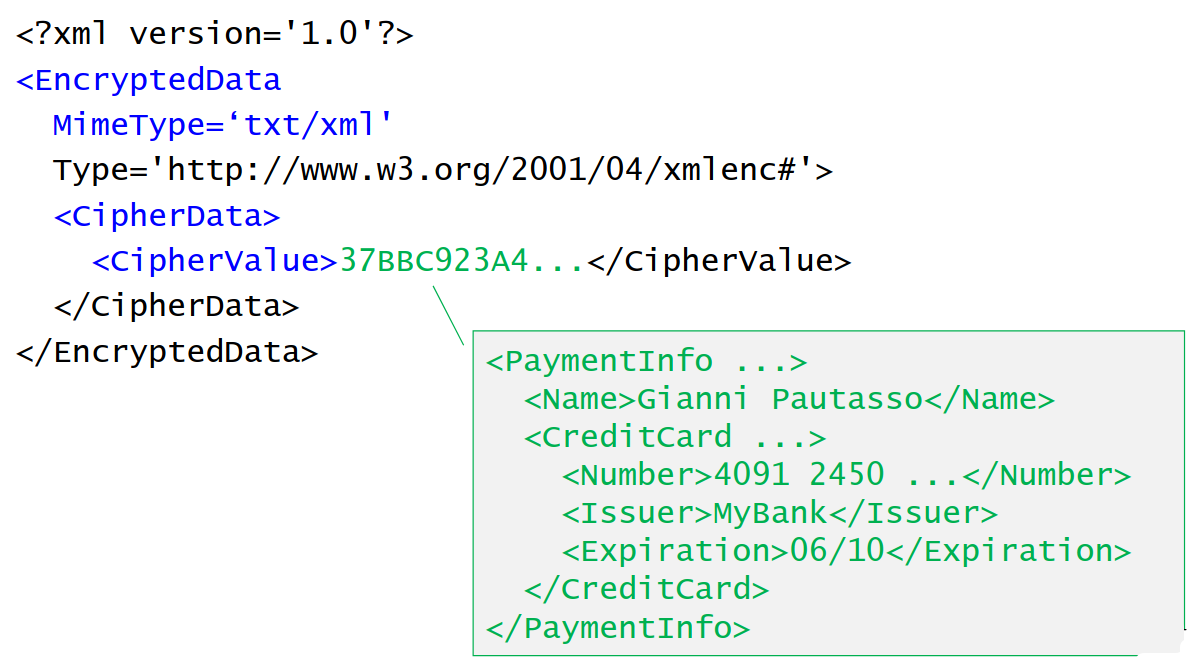
\includegraphics[width=0.48\textwidth]{img/xml encryption ex 3.png}\label{fig:xml enc ex 3}}
  \hfill
  \subfloat[XML Encryption Example 4]{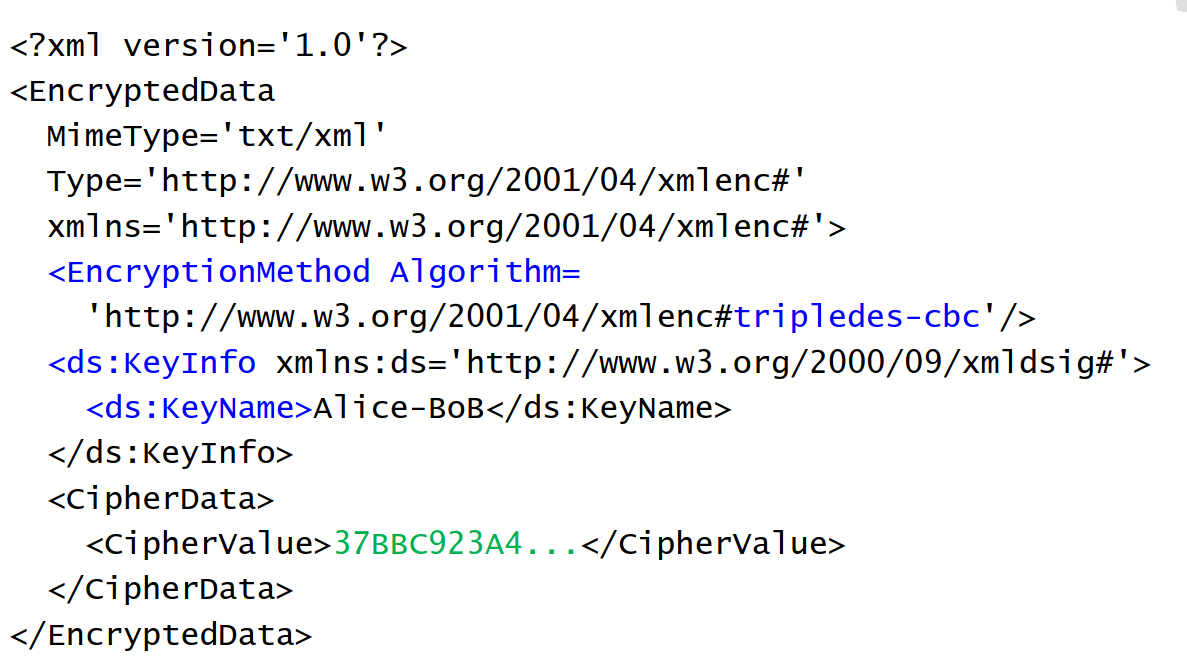
\includegraphics[width=0.48\textwidth]{img/xml encryption ex 4.png}\label{fig:xml enc ex 4}}
  \caption{XML Encryption Examples}
  \label{fig:xml enc ex}
\end{figure}
